\newpage
\begin{center}
  \textbf{\large 2. СРАВНЕНИЕ КАЧЕСТВА РАБОТЫ СУЩЕСТВУЮЩИХ МЕТОДОВ}
\end{center}
\refstepcounter{chapter}
\addcontentsline{toc}{chapter}{2. СРАВНЕНИЕ КАЧЕСТВА РАБОТЫ СУЩЕСТВУЮЩИХ МЕТОДОВ}

\section{Данные для обучения}

Немаловажной частью для области машинного обучения являются данные, на которых это всё обучается и оценивается.
Без различных разбиений данных становится невозможно детектирование переобучения.
Без качественных и репрезентативных данных нельзя построить эффективный алгоритм, который будет способен решать реальные задачи.
Чем лучше подобран датасет, тем точнее и надежнее будет работать модель.
Качество датасета определяется не только объемом.
Необходимо, чтобы данные отражали все возможные сценарии, с которыми модель столкнется в реальном мире, иначе могут возникнуть проблемы с переобучением или недообучением, что снизит качество предсказаний.
Несбалансированные данные могут привести к тому, что модель будет хуже предсказывать редкие классы, а наличие ошибок в разметке исказит результаты обучения.
Разнообразие датасетов — это еще один критически важный аспект.
Так данные аудио данные для обучения модели распознавания речи на различные темы не могут состоять исключительно из аудиокниг.
Таким образом, датасеты — это фундамент машинного обучения, от которого зависит успех всего проекта и который вляет на способность модели принимать правильные решения в реальных условиях.
Существует огромное количество самых различных датасетов, которые содержат аудио записи, относящиеся  к разным тематикам.
Поговорим сначала об английских.

LibriSpeech -- это один из наиболее значимых и широко используемых датасетов в области обработки речи, который какое-то время был самым большим и разнообразным набором данных.
Он содержит в себе озвученные профессиональными спикерами аудиокниги.
Его важность заключается в том, что он предоставляет большой объем размеченных данных, что критически необходимо для обучения и оценки моделей машинного обучения.
Существуют вариации разбиения на 100, 360 и 500 часов.
Также датасет разбивается на clean и other.
Первый проще для распознавания речи, второй сложнее.
Наличие нескольких вариантов разбивки помогает оценивать устойчивость моделей к разному уровню шумов и качеству записи.
Это особенно важно, поскольку в реальных условиях системы распознавания речи сталкиваются с разнообразными акустическими условиями, и датасет должен отражать эту вариативность.

Еще одна важная особенность Librispeech -- его открытость и доступность.
Это позволяет академическим исследователям и небольшим стартапам работать с качественными данными без необходимости сбора собственного корпуса, что требует значительных временных и финансовых затрат, о чём мы говорили ранее в первой главе.
Благодаря этому датасету, разработка технологий распознавания речи стала более доступной для широкого круга специалистов.

Common Voice на данный момент один из крупнейших датасет и самых популярных набор данных.
Это масштабный открытый проект компании Mozilla, направленный на создание общедоступного датасета для обучения систем распознавания речи. 
Он собирается и проверяется силами волонтёров по всему миру, благодаря чему он обладает огромным и разнообразным корпусом пар ауидо-текст.
Ещё он содержит разнообразные темы, а также сотни вариантов произношения.
Такое множество вариантов позволит оценить общую точность работы моделей и подходов.
Каждый человек после регистрации может  внести свой вклад несколькими способами:
\begin{itemize}
  \item Пожертвовать фразу для озвучивания с указанием источника, например книги, газеты и так далее.
    Или же условные фразеологизмы.
  \item Озвучить фразы из общего пула, которые выбираются случайным образом.
  \item Проверить фразы на правописание.
  \item Проверить качество озвучки фраз, чтобы отбросить сгенерированные или плохо озвученные.
\end{itemize}
Весь набор данных предоставляется бесплатно при соглашение на условия.
В отличие от многих других датасетов, которые часто ограничены дикторами с определенным акцентом или языком, Common Voice охватывает десятки языков, включая редкие и малоресурсные, что крайне важно для разработки голосовых технологий, доступных всем пользователям.
Все записи в Common Voice доступны под свободной лицензией CC-0, что позволяет использовать их без юридических ограничений как в академических исследованиях, так и в коммерческих продуктах.
Это особенно ценно для стартапов и небольших компаний, у которых нет ресурсов для сбора собственных данных.
Кроме того, датасет включает метаданные, такие как возраст, пол и регион говорящего, что позволяет обучать более адаптивные и справедливые модели, минимизируя смещения, а также проводить аудиоаналитику и более детальную оценку.

Еще одно преимущество Common Voice — его постоянное расширение и обновление. Поскольку проект краудсорсинговый, сообщество регулярно добавляет новые записи, улучшая покрытие разных акцентов, диалектов и демографических групп.
Common Voice также играет важную роль в развитии open-source технологий.
Многие современные проекты используют этот датасет для обучения и тестирования, что способствует созданию более доступных и прозрачных решений в области искусственного интеллекта.
Благодаря своей открытой природе проект помогает снизить зависимость от проприетарных датасетов, которые часто ограничивают развитие независимых исследований.
Таким образом, Common Voice -- важная часть области распознавания речи, которая делает технологии транскрибации ауидо более доступными.
Его разнообразие, открытость и постоянное развитие помогают преодолевать языковые барьеры и создавать голосовые системы, способные понимать людей по всему миру, независимо от их языка или акцента.

\begin{figure}[!t]
  \centering
  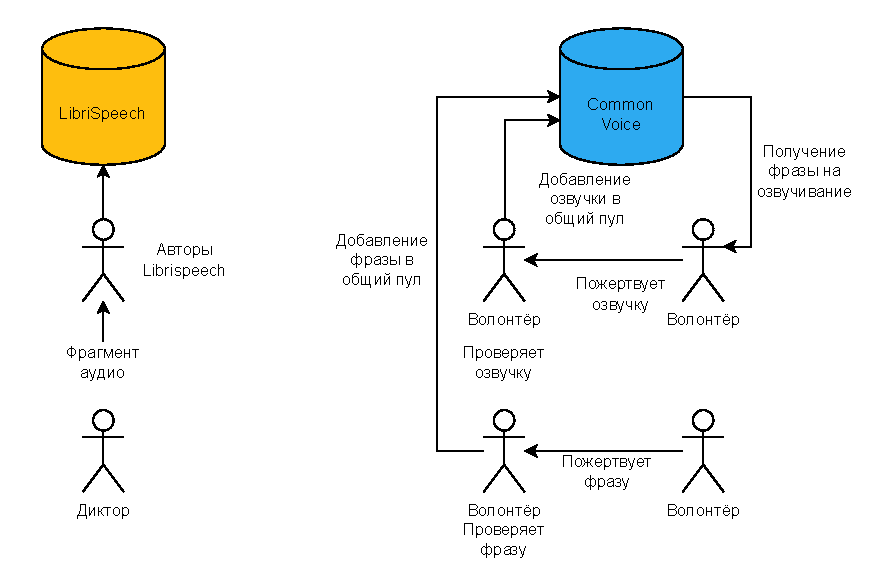
\includegraphics[width=160mm]{LS_CV.pdf}
  \caption{Устройство сбора датасетов LibriSpeech и Common Voice.}
  \label{fig:ls_cv}
\end{figure}

Эти датасеты являются наиболее разнообразными по темам и набору спикеров, поэтому оценка качества распознавания для английского языка в основном проводится для них.
Общий вид получения данных для этих датасетов можно найти на Рис.~\ref{fig:ls_cv}.
Для русского языка существуют свои русские версии вышеупомянутых LibriSpeech и Common Voice.
Также существуют несколько датасетов, собранных чисто для русского языка. 
Например,набор данных от создателей SeleroVAD - OpenSTT. 
Он покрывает разные темы: 
\begin{enumerate}
  \item Радиоэфиры
  \item Аудиокниги
  \item Телефонных разговоров
  \item Публичных выступлений
  \item Видео с ютуба
\end{enumerate}
Именно YouTube, как часть датасета играет особую роль в развитии систем ASR, так как отражает реальные условия использования, с которыми сталкиваются современные голосовые технологии.
В отличие от студийных записей или аудиокниг, YouTube-ролики содержат естественную речь с разнообразными акцентами, тембрами голосов, фоновыми шумами и неоднородным качеством звука. 
Кроме того, YouTube-данные в OpenSTT помогают решать проблему «domain shift» — ситуации, когда модель, обученная на идеальных данных, плохо работает с реальными записями.
Например, системы, тренированные только на аудиокнигах, часто ошибаются при обработке спонтанной речи с паузами, междометиями или перекрывающимися репликами.
YouTube-сегмент датасета смягчает эту проблему, так как включает подобные сценарии, улучшая способность модели обобщать знания.

Мы выберем 21 версию Common Voice (последнюю на момент написания) для русского языка.
Такая фиксация необходима, так как датасет постоянно обновляется, о чём было написано выше.
Дополнительно мы оставим только верифицированные аудиозаписи, чтобы отбросить потенциально плохие данные.

\section{Выбор моделей}
\subsection{ASR}

В качестве основных моделей для тестирования мы определим от Nvidia FastConformer, обученный для русского языка и Whisper Large от OpenAI, упомянутые в первой главе.
Почему эти две модели? Основная причина -- их непохожесть.

Обе модели построенны на разных архитектурах, имеют отличие в размерах в 10 раз, одна является заточенной под один язык, а другая мультиязычной.
Это важно потому, что в реальных задачах модели могут сильно различаться по своей структуре, принципам работы и особенностям обучения, и метод, который хорошо работает на одной архитектуре, может оказаться бесполезным или даже вредным для другой.
Также эффективность алгоритма может  зависить от разных факторов, таких как качество аудиозаписи, например.
Тестирование на разнородных моделях позволяет выявить скрытые зависимости и ограничения метода.
Еще один важный аспект -- воспроизводимость результатов.
Чтобы избежать проблем, необходимо проводить кросс-архитектурное тестирование, которое подтвердит, что улучшение не является артефактом экспериментальной setup-а или особенностей конкретной модели.
Использование именно этих двух моделей позволит сравнить работу некоторых методов на двух моделях сразу, а также далее в 3 главе позволит проверить идею переноса способности к коррекции ошибок между настолько разными моделями.

Также преимуществом именно этих двух моделей являются обширная документация, которая поможет в проведение опытов, и наличие большой базы пользователей, которая разбирала ошибки и также проводила свои эксперименты.
Наличие качественной документации и активного сообщества, предлагающего множество готовых решений, значительно упрощает и ускоряет процесс разработки в машинном обучении. Хорошая документация выполняет роль фундамента, на котором строится понимание инструментов, библиотек и методов. Она позволяет разработчикам быстро осваивать новые технологии, избегая необходимости разбираться во внутренней реализации с нуля.
Когда тысячи разработчиков используют одни и те же инструменты, проблемы выявляются и фиксируются гораздо оперативнее, чем в закрытых или малораспространенных системах.
Тем самым повышается надежность решений и снижает риски, связанные с использованием новых или экспериментальных методов.
Ещё сообщество часто разрабатывает дополнительные утилиты и надстройки, расширяющие базовый функционал и адаптирующие его под специфические нужды.

Ну третьим преимуществом является то, что данные модели выпускались более полутора лет назад, а значит они гарантированно не видели части данных из наших тестовых наборов данных.
Так решается проблема утечки данных из обучающей выборки в тестовую (data leakage).

\subsection{Коррекция}

В качестве способов улучшения качества мы используем BeamSearch декодирование, выравнивание гипотез с помощью статистических методов ROVER и рескоринга с помощью языковой модели.
Эти 3 метода имеют:
\begin{itemize}
  \item Низкую вычислительную нагрузку сверху.ы
  \item 2/3 могут быть применены к разным ASR без необходимости переобучения.
\end{itemize}

В качестве языковой модели мы используем n-gram модель, обученной с помощью KenLM.
Преимуществом в нашем случае является то, что достаточно легко можно найти гайд на обучение и на интеграцию модели с FastConformer.
В качестве текстового набора данных мы используем русский сплит mc4 датасета, который содержит большой набор данных, собраный с интернета парсерами.
mC4 -- мощный инструмент для n-граммного моделирования.
Его главные преимущества -- масштаб, наличие русского сплита и интеграция с KenLM.
Датсет поддерживает расчёт перплексии через предобученные 5-граммные модели KenLM, что упрощает фильтрацию текстов по качеству.
Ещё это может быть использовано для калибровки параметров сглаживания n-грамм.
Недостатком же выступает то, что, несмотря на очистку, веб-тексты могут содержать опечатки или несогласованные n-граммы.
Гиперпараметр количества n-граммов мы укажем равным 4.

\section{Результаты существующих методов}

\begin{table}[]
\centering
\caption{Сравнение значений WER среди отобранных существующих методов.}
\begin{tabular}{|c|c|ccc|}
\hline
\multirow{2}{*}{Модель}        & \multirow{2}{*}{Сеттинг}             & \multicolumn{3}{c|}{Датасет, WER}                                    \\ \cline{3-5} 
                               &                                      & \multicolumn{1}{c|}{CV21}  & \multicolumn{1}{c|}{RuLS}     & OpenSTT \\ \hline
\multirow{4}{*}{FastConformer} & Greedy                               & \multicolumn{1}{c|}{12.31} & \multicolumn{1}{c|}{38.43}    & 25.13   \\ \cline{2-5} 
                               & BeamSearch                           & \multicolumn{1}{c|}{12.26} & \multicolumn{1}{c|}{38.84}    & 25.07   \\ \cline{2-5}
                               & ROVER                                & \multicolumn{1}{c|}{13.50} & \multicolumn{1}{c|}{37.78}    & 28.54   \\ \cline{2-5}
                               & LM                                   & \multicolumn{1}{c|}{9.87}  & \multicolumn{1}{c|}{37.18}    & 27.28   \\ \hline 
\multirow{3}{*}{Whisper}       & Greedy                               & \multicolumn{1}{c|}{19.60} & \multicolumn{1}{c|}{37.89}    & 24.38   \\ \cline{2-5} 
                               & BeamSearch                           & \multicolumn{1}{c|}{18.33} & \multicolumn{1}{c|}{35.49}    & 24.19   \\ \cline{2-5}
                               & ROVER                                & \multicolumn{1}{c|}{23.16} & \multicolumn{1}{c|}{39.05}    & 29.90   \\ \hline
                               
\end{tabular}
\label{tab:res_base}
\end{table}

Важная оговорка, которую стоит сделать -- результаты на OpenSTT считаются без пунктуации и с переводом слов в нижний регистр.
Сделано это из-за того, что приведённые транскрипции записаны в таком виде.

Как мы видим в Таблице~\ref{tab:res_base}, только LM принесла прирост в качестве на наших данных, уменьшив WER на 20\% на Common Voice 21.
BeamSearch отработал с приростом на Common Voice, но на RuLibriSpeech значение ошибки выросло у FastConformer модели.
Здесь же и отличие от Whisper -- у последнего использования методики декодирования BeamSearch привело к улучшению результатов декодирования на всех трёх наборах данных.
ROVER дал прирост исключительно для Whisper на датасете LibriSpeech, но в целом, учитывая, что он по факту берёт просто самый вероятный токен и при этом является самым легковесным методом, ожидаемо.
Естественно, это с оговоркой, что ему для работы необходимо сгенерировать гипотезы с помощью BeamSearch.
Также, несмотря на то, что модель FastConformer была заточена под распознавания только русского языка, но на RuLibrispeech модель показала себя незначительно хуже в сравнение c моделью Whisper от OpenAI.
Хотя на том же CV 21 модель Nvidia показывает себя лучше, несмотря на разницу в 10 раз в количестве параметров.

Более подробно примеры мы разберём в следующей главе.

\section{Выводы}
В данной главе была проведена экспериментальная оценка нескольких легковесных методов улучшения качества распознавания речи.
Результаты работы методов представлены на 3 выбранных русскоязынчных датасетах - Common Voice, RuLibriSpeech и OpenSTT YouTube-val-700
Были выявлены отличия между наборами данным.